%! suppress = EscapeUnderscore
%! Author = Leonardo Cruciani
%! Date = 29/03/2025

% Preamble
\documentclass[11pt]{article}

% Packages
\usepackage[top=1in, bottom=1.2in, left=1in, right=1in]{geometry}
\usepackage{amsmath}
\usepackage{upgreek}
\usepackage{graphicx}
\usepackage{wrapfig}
\usepackage{hyperref}
\usepackage{amsfonts}
\usepackage{listings}
\newcommand{\atan}{\,\mathrm{atan}}
\newcommand{\sgn}{\,\mathrm{sgn}}
\newcommand{\pdf}{\,\mathrm{pdf}}
\usepackage{cite}

\usepackage[backend=biber,style=authoryear,]{biblatex}
\addbibresource{bibliography.bib} %Imports bibliography file

\author{Leonardo Cruciani}
\title{Forecasting VaR using GARCH and KDE}
% Document
\begin{document}
    \maketitle
    \section{Introduction}
    \label{sec:introduction}
    Modeling and forecasting risk is a cornerstone of financial econometrics.
    Among risk measures, Value-at-Risk (VaR) is one of the most widely used tools for quantifying potential losses in portfolios over a given time horizon and confidence level, as discussed in \textcite{jorion2006value}.
    However, the accuracy of VaR depends critically on how well the distribution of returns is modeled, especially in the tails.
    Financial returns typically exhibit heavy tails, skewness, and volatility clustering—features that violate the assumptions of normality underlying classical VaR approaches like RiskMetrics.
    To address these stylized facts, the paper by~\textcite{thorsten} proposes a \textit{scale-consistent} VaR framework that combines truncated skewed Lévy distributions (TSL) with an augmented GARCH volatility modeling~\parencite{pagan1990alternative}.
    This approach captures both the time-varying volatility and non-Gaussian behavior of asset returns and improves longer horizon VaR forecasting through a scaling rule derived from Lévy flight dynamics.
    In this paper, I first (sections~\ref{sec:GARCH} and~\ref{sec:replication}) replicate the method of~\textcite{thorsten} to forecast Value-at-Risk using GARCH-filtered returns modeled with a truncated skewed Lévy distribution.
    Here, I use Kernel Density Estimation (KDE)~\parencite{silverman1986density} to improve the computational complexity of the task of calibrating the TSL shape parameters.
    The accuracy of the VaR estimates is evaluated by means of a backtesting procedure based on the number of breaches, following the methodology proposed in \textcite{christoffersen2003elements}.
    Then (in section~\ref{sec:direct}), motivated by the rigidity of parametric approaches, I introduce a nonparametric alternative based on empirical quantiles and drop the TSL distribution assumption.
    This nonparametric approach offers both advantages and disadvantages: it requires fewer distributional assumptions, is relatively easy to implement and offers overall better results, but at the expense of requiring more data for empirical quantiles to accurately estimate their true values.

   \section{Data}\label{sec:data}
    The dataset contains the closing prices of the S\&P500 index from 2006 to 2024.
    The dataset is split in two, with the first 11 years being used for training and the last 7 years for testing.
    From the dataset the log returns are computed, expressed in percentage terms, and aggregated for 5, 10 and 20 days.

    \section{GARCH}
        \label{sec:GARCH}
        The paper~\textcite{thorsten} uses an augmented GARCH model that nests some of the most commonly used (e.g.\ GARCH(1,1), GJR-GARCH, Aparch, etc.) generalizations.
        In this work I will resort to a simpler Power GARCH model with leverage effect to model the volatility $\sigma_t$:
        \begin{equation}
            \label{eq:model}
            \sigma_t^\kappa = \omega + \gamma \left|\epsilon_{t-1}\right|^\kappa + \delta \sigma_{t-1}^\kappa + \eta \left|\epsilon_{t-1}\right|^\kappa I_{[\epsilon_{t-1}<0]}
        \end{equation}
        Where $\epsilon_t \sim D(0,1)$ are independent shocks distributed according to a \textit{standardized distribution} $D(0,1)$.
        In the paper~\textcite{thorsten} and in section~\ref{sec:replication} this $D(0,1)$ distribution is the TSL calibrated on historical data, while in section~\ref{sec:direct} the KDE distribution is used.
        The parameters to be estimated are: $\gamma$, which models the sensitivity of the volatility to the shock; $\delta$, which models the persistence of the volatility; $\eta$, which models the leverage effect; the exponent $\kappa$ (typically $\simeq 2$) and the so called (when $\kappa=2$) long term variance $\omega$.\\
        To model the return $r_t$ I used the following model:
        \begin{equation}
                r_t = \mu + \sigma_t \epsilon_t,
                \label{eq:return_equation}
        \end{equation}
        Where the mean $\mu$ can be safely assumed to be constant for medium to short term returns.
        The parameters of the GARCH are calibrated on historical data and the model is then used to forecast the next period variance $\hat \sigma_{t+1}^2$ as returns become available.
        Therefore, the closing prices in the dataset are standardized following the formula:
        \begin{equation}
            z_t = \frac{r_t - \hat \mu}{\hat \sigma_t}
            \label{eq:standardization_equation}
        \end{equation}
        where $\hat \mu$ and $\hat \sigma$ are obtained from the GARCH\@.
        \input{GARCH}

    \section{Paper Replication}
    \label{sec:replication}
        \subsection{Truncated Skewed Levy}\label{subsec:truncated-skewed-levy}
    The $TSL(\mu, c, \alpha, \lambda, \beta)$ is defined through  its characteristic function $\varphi_{TSL}(k) = \exp\big(-\psi(k; \mu, c, \alpha, \lambda, \beta)\big)$ where:
        \begin{equation}
            \begin{aligned}
                \psi(k; \mu, c, \alpha, \lambda, \beta) &= ik\mu \,+\\
                                                    & + c^{\alpha}\left[\frac{\lambda^2-(k^2+\lambda^2)^{\alpha/2}}{\cos(\pi \alpha/2)}\cos\left(\alpha \atan \left(\frac{|k|}{\lambda}\right)\right)\right] \times \\
                                                    & \times \left[ 1+ i \sgn(k) \beta \tan \left(\alpha\left(\frac{|k|}{\lambda}\right)\right) \right]
            \end{aligned}\label{eq:char_func}
        \end{equation}
        for all $k \in \mathbb{R}$.
        The parameters have the following meaning (see figure~\ref{fig:parameters}):
        \begin{itemize}
            \item $\mu$ is the location parameter.
            \item $c >0$ is the scale parameter.
            \item $\alpha \in (0,2] \setminus\{1\} $ is the characteristic exponent, which defines the overall shape of the PDF, and especially the fatness of the tails.
            To give an intuition, the closer $\alpha$ is to $2$, the closer the $TSL$ approximates a Gaussian.
            \item $\lambda > 0$ is the cutoff parameter, which is responsible for making the moments of the TSL well-defined.
            \item $\beta \in [-1, 1]$ is the skewness parameter: the PDF of the TSL is skewed to the right for negative $\beta$ and to the left for positive $\beta$.
        \end{itemize}
        The PDF of the distribution can be obtained by fourier transforming the characteristic function:
        \begin{equation}
            \pdf_{TSL}(x; \mu, c, \alpha, \lambda, \beta) =  \frac{1}{2\pi}\int_{\mathbb R} \exp\big(-ikx-\psi(k; \mu, c, \alpha, \lambda, \beta)\big)\,dk\label{eq:pdf}
        \end{equation}
        \begin{figure}[h!]
            \label{fig:parameters}
            \centering
            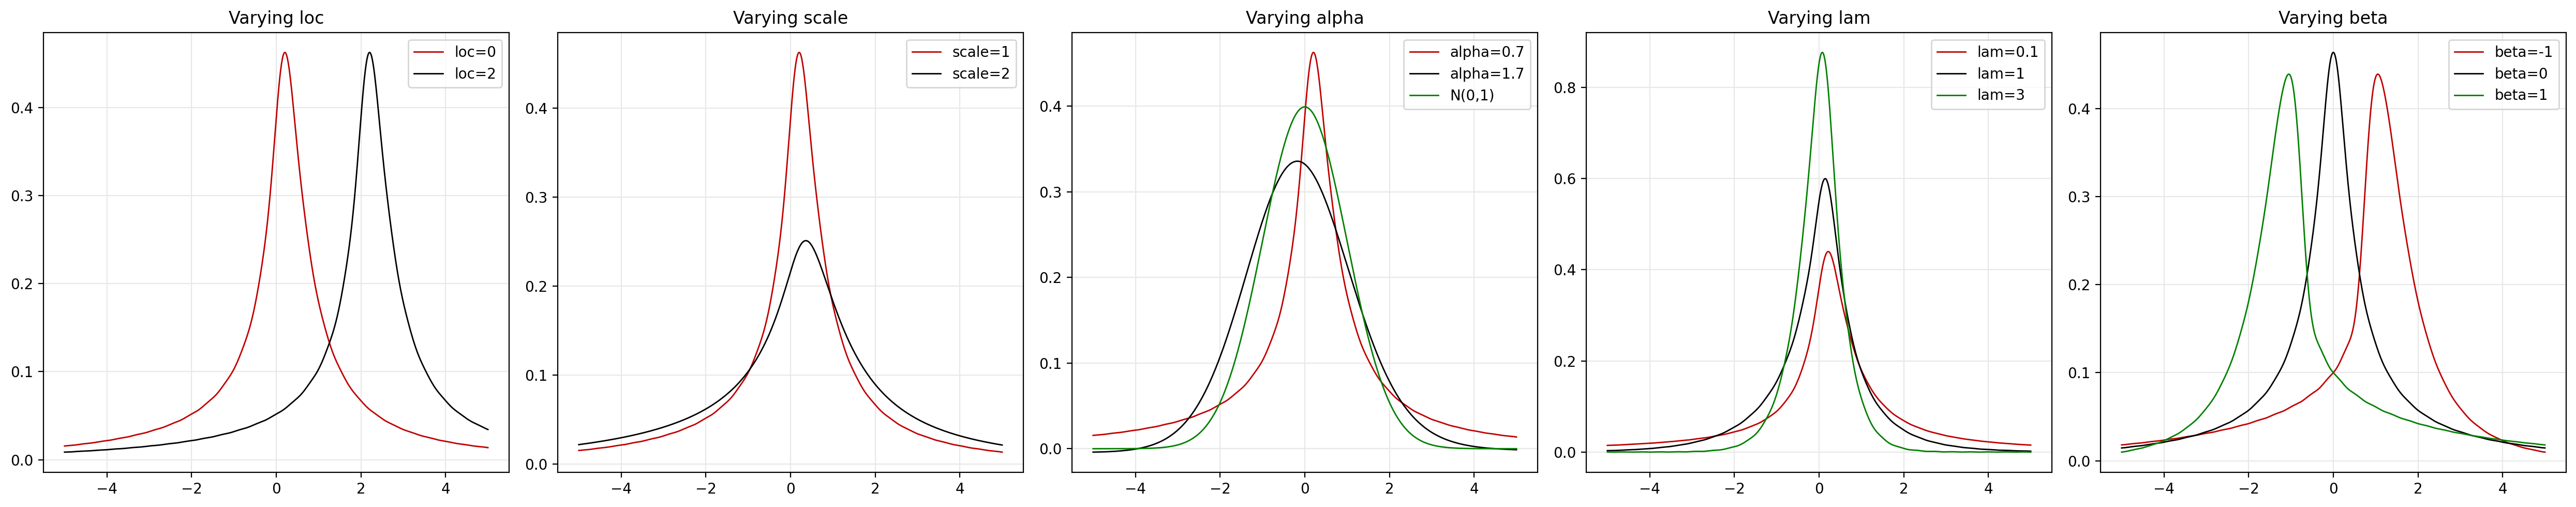
\includegraphics[width=0.9 \linewidth]{img/parameters}
            \caption{TSL PDF. Baseline parameters: $\mu=0, \,c=1,\, \alpha = 0.7, \, \lambda = 0.2,\, \beta =-0.2$}
        \end{figure}
        The fundamental property of this distribution which makes it well suited for the task of estimating longer horizon variances is its convolution property.
        In particular the $T$-day convolution of the PDF satisfies:
        \begin{equation}
            \pdf^T_{TSL}(x; \lambda) = T^{-1/\alpha} \pdf_{TSL}\left(T^{-1/\alpha} x; T^{1/\alpha}\lambda\right).
            \label{eq:scaling}
        \end{equation}
        Therefore, by fitting the TSL distribution parameters on daily returns and appropriately scaling the PDF, we can approximate the distribution of larger horizon returns.

        \begin{figure}[h!]
            \centering
            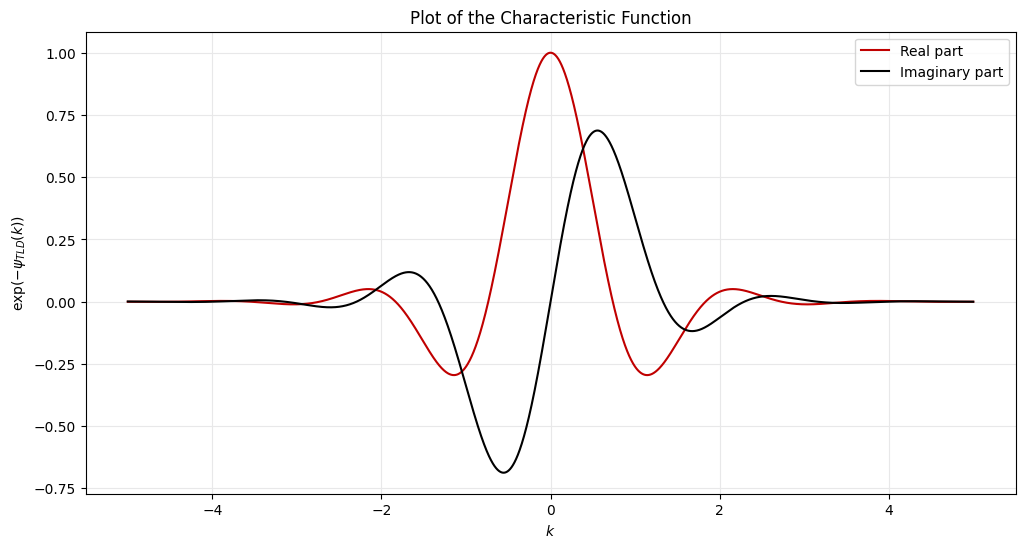
\includegraphics[width=0.6 \linewidth]{img/char_func}
            \caption{The characteristic function of the TSL. Parameters: $\mu=2, \,c=5,\, \alpha = 0.7, \, \lambda = 2,\, \beta =-0.8$}
            \label{fig:char_func}
        \end{figure}

        \subsection{Fitting the TSL}\label{subsec:fitting-the-tsl}
    To obtain the PDF, the characteristic function (see figure~\ref{fig:char_func}) must be numerically Fourier-transformed.
        Following the paper approach, we use Romberg integration for $k \in [-15, 15]$ using $2^{12}+1$ steps.
        This calculation is computationally expensive: for a given set of the five parameters, evaluating the PDF for 1000 $x$ points takes around 5 seconds.
        As the dataset contains around 7000 observations, the calculation of the loglikelihood for a given parameter set takes around 35 seconds, or in other words,
        even a simple grid search over the parameters $\alpha, \lambda, \beta$ (as we are fitting on standardized returns, we can assume $\mu=0, c=1$) with a $7\times 7\times 7$ grid would take around 3.5 hours to complete.
        Therefore, I resorted to a faster, but less accurate approach:
        \begin{enumerate}
            \item I compute the KDE PDF of the standardized returns with bandwidth parameter given by Scott’s rule of thumb:
                    $$b = n^{-1/5}$$
            \item I evaluate the KDE PDF in a symmetric, log-spaced grid (denser around $0$) of $201$ points for $x\in [-15,15]$.
            \item I perform a grid search to find the set of parameters $\alpha, \lambda, \beta$ that minimizes the total squared error
                between the KDE PDE and the TSL PDF calculated with the given set of parameters on the points in the log-spaced grid,
                effectively reducing the number of required calls to the TSL PDF to $201$ for each parameter set.
                The grid was chosen by taking 13 equally spaced points in the following ranges:
                $$ \alpha \in [0.75,0.81], \quad \lambda \in [1.60,1.80], \quad \beta \in [-0.18,-0.12].$$
        \end{enumerate}
        In figure~\ref{fig:fitted_tls}, we see a plot of the resulting TSL PDF and in table~\ref{tab:parameters} we see the results of the grid search.\\
        Unfortunately this approach is not free of consequences in terms of accuracy, as the total mean squared error (TMSE) of the KDE PDF greatly dominates the total squared error of the grid search:
        \begin{equation}
            \begin{aligned}
                &\widehat{TMSE}_{KDE} = \frac{1}{2\sqrt{\pi}} \sum_{i=1}^{201}\widehat{\pdf}_{KDE}(x_i) = 1.88, \\
                &\widehat{TSE}_{GS} = \sum_{i=1}^{201}\bigg(\pdf_{TSL}(x_i, \hat{\alpha}, \hat{\lambda}, \hat{\beta})-\widehat{\pdf}_{KDE}(x_i)\bigg)^2 = 0.005,
            \end{aligned}
            \label{eq:errors}
        \end{equation}
        and the errors in table~\ref{tab:parameters} are likely to severely underestimate the actual standard errors of $\hat{\alpha}, \hat{\lambda}, \hat{\beta}$ if treated as estimators of the parameters of the actual distribution of the data.

        \begin{table}[h!]
            \centering
            \begin{tabular}{l|ccc}
                \textbf{Parameters} & $\hat \alpha$ & $\hat \lambda$ & $\hat \beta$  \\
                \hline
                 \textbf{Values} & 0.765 & 1.67 & -0.155\\
                \textbf{Absolute Errors} & 0.005 & 0.01 & 0.005 \\
                \textbf{Standard Errors} & 0.002 & 0.006 & 0.002 \\
            \end{tabular}
            \caption{The SE have been calculated assuming a uniform distribution in the interval where the estimate lies, and thus dividing the absolute errors by $\sqrt{3}$.
            Note: These errors refer to the parameter values used to fit the KDE approximation, and do not reflect confidence intervals for the true underlying distribution.}
            \label{tab:parameters}
        \end{table}

        \begin{figure}[h!]
            \centering
            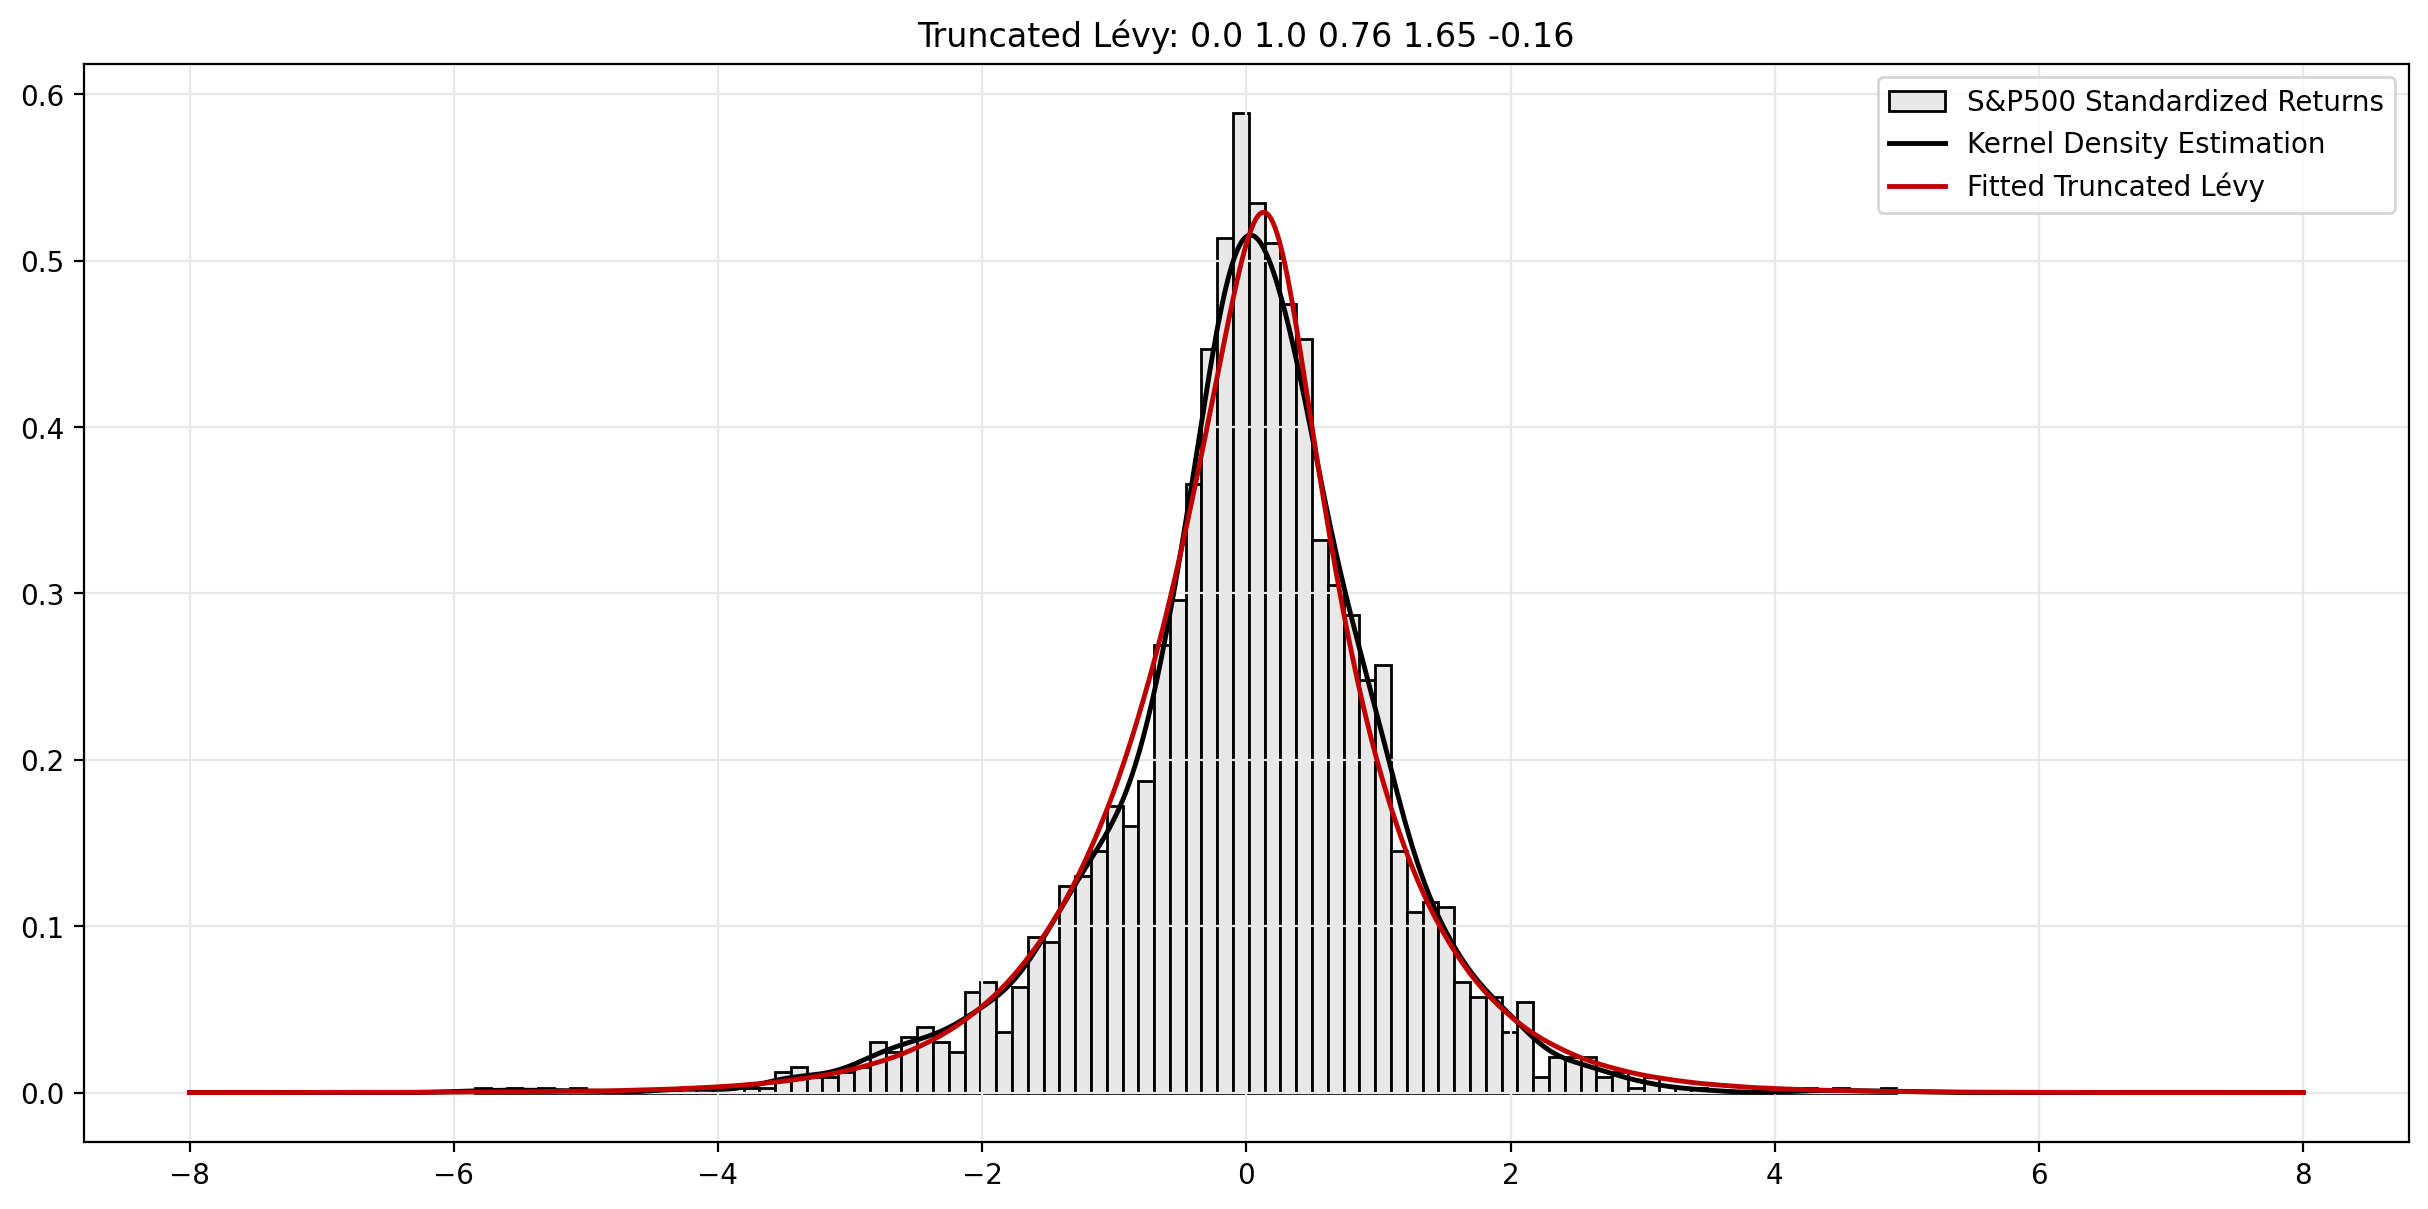
\includegraphics[width=0.6 \linewidth]{img/fitted_tls}
            \caption{TSL PDF obtained by calibrating the parameters over the KDE PDF, and the standardized returns.}
            \label{fig:fitted_tls}
        \end{figure}

        \subsection{Estimating the 1-Day VaR}\label{subsec:estimating-the-1-day-var2}
    I then proceed to calculate the 1st, 5th and 10th percentiles of the (1-Day) distribution $D(0,1)=TSL(0,1,\hat \alpha,\hat \lambda,\hat \beta)$ numerically:
        $$ Q(0.01) = -2.96, \quad Q(0.05) = -1.79, \quad Q(0.1) = -1.26  $$
        The $N$\% 1-Day VaR is then obtained by multiplying the volatilities obtained from the GARCH by the $N$th percentile of the distribution.
        \begin{equation}
            VaR_t(N\%) = -Q(N\%) \, \sigma_t.
        \end{equation}
        We define a \textit{breach} a trading day when the realized return $r_t$ is more negative than the minus VaR:
        \begin{equation}
            r_t < - VaR_t(N\%)
        \end{equation}
        For the VaR estimate to be valid, over a time interval large enough the percentage of breach day should tend to $N\%$.
        In figure~\ref{fig:1_day_var} we can see the minus 1\% 1-Day VaR for the S\&P500 compared to its daily returns.
        We achieved a reasonable amount of breaches in both the training (on which the model is calibrated) and the test set.
        The results are shown in table~\ref{tab:var_breaches}.

        \begin{figure}[h!]
            \centering
            \label{fig:1_day_var}
            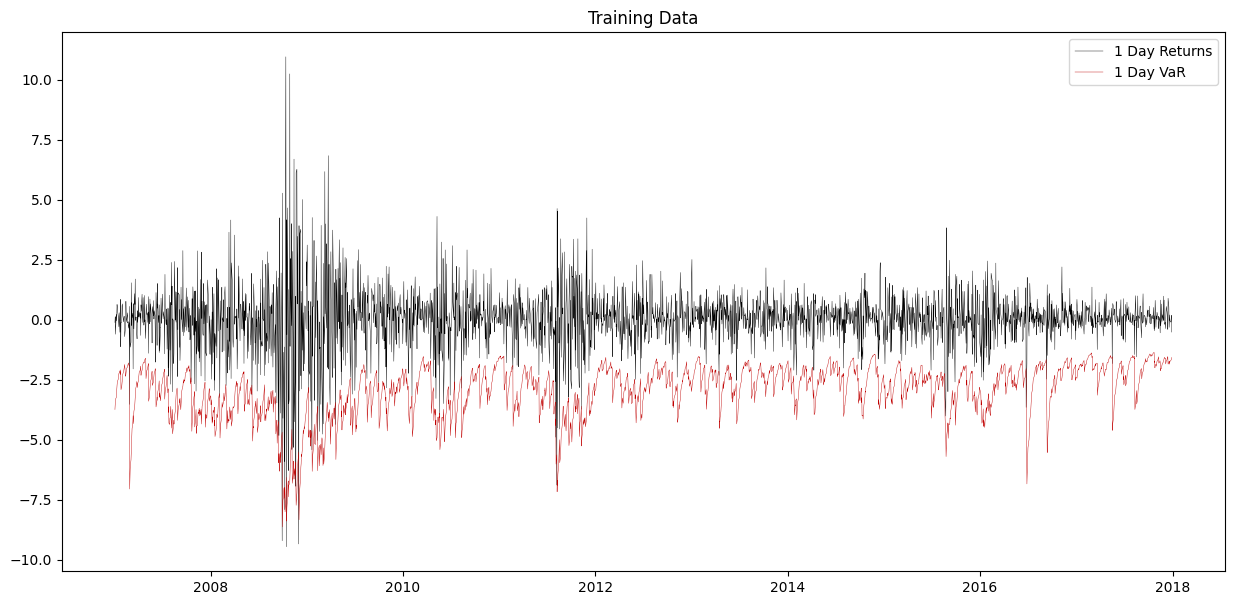
\includegraphics[width=0.8\linewidth]{img/train1}
            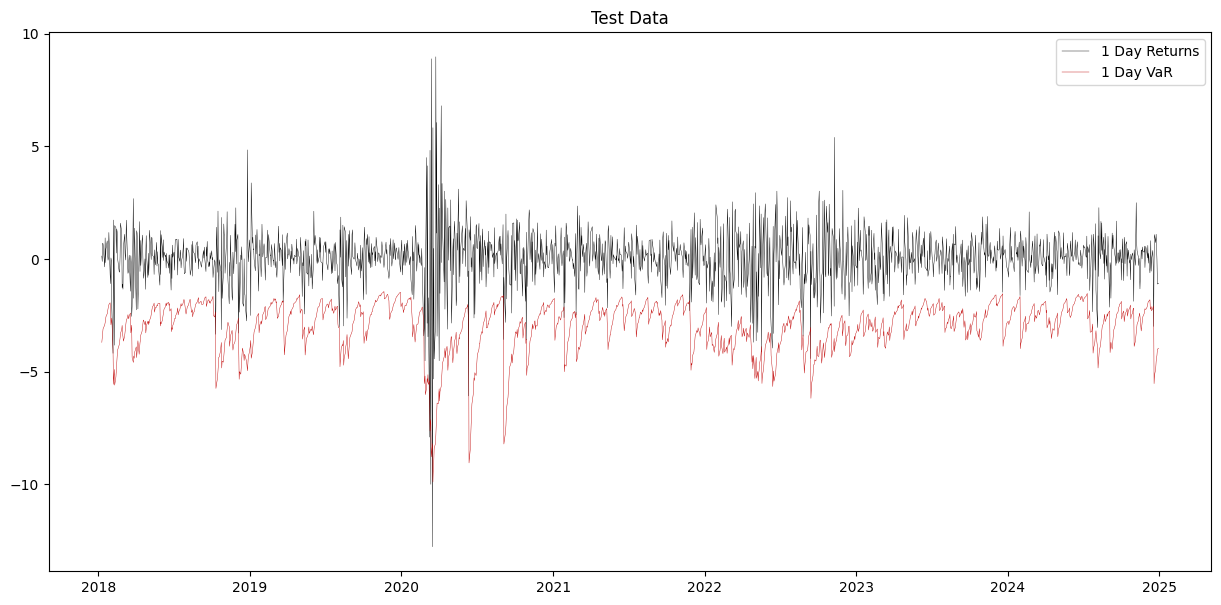
\includegraphics[width=0.8\linewidth]{img/test1}
            \caption{S\&P500 1\% 1-Day VaR and its daily returns}
        \end{figure}

        \begin{table}[h!]
            \centering
            \begin{tabular}{l|cc}
                  \textbf{VaR}   & \textbf{Training} & \textbf{Test} \\
                  \hline
                  1\%   & 0.94\% & 1.02\% \\
                  5\%   & 5.16\% & 4.56\% \\
                  10\%  & 9.82\% & 9.54\% \\
            \end{tabular}
            \caption{Daily VaR breaches in the S\&P500}
            \label{tab:var_breaches}
        \end{table}

        \subsection{Estimating the 10-Day VaR}
        A similar procedure is repeated to estimate the 10-Day VaR. Taking advantage of the TSL convolution properties, we evaluate the quantiles of $D(0,N^{1/\hat{\alpha}}) = TSL(0,1,\hat \alpha,N^{1/\hat{\alpha}},\hat \lambda,\hat \beta)$, to find:
        $$Q_{10}(0.01) =  -8.11, \quad Q_{10}(0.05) = -5.56, \quad Q_{10}(0.1) = -4.26$$
        We thus calculate the 10-Days VaR by multiplying the quantile to the daily volatility, and we calculate the breaches, which are found in table~\ref{tab:var_breaches}.
        \begin{table}[h!]
            \centering
            \begin{tabular}{l|cc}
                  \textbf{VaR}   & \textbf{Training} & \textbf{Test} \\
                  \hline
                  1\%   & 1.05\% & 2.22\% \\
                  5\%   & 4.01\% & 5.58\% \\
                  10\%  & 6.7 \% & 8.68\% \\
            \end{tabular}
            \caption{10 Days VaR breaches in the S\&P500}
            \label{tab:scaled_var_breaches}
        \end{table}

    \section{Direct Method} \label{sec:direct}
    In this section I get rid of any assumption on the standardized return distribution, and opt for a full nonparametric approach,
    by directly estimating the empirical quantiles from the standardized data:
    \begin{equation}
        \hat Q_p(x) = x_{\lfloor h \rfloor} + (h-\lfloor h \rfloor) (x_{\lceil h \rceil}-x_{\lfloor h \rfloor}), \quad h = (N-1)p+1.
        \label{eq:empirical_quantiles}
    \end{equation}
    This estimator is consistent and asymptotically normal~\parencite{david2003order}:
    \begin{equation}
        \sqrt{N}\left( \hat Q_p(x) - x_p \right)\xrightarrow{d} N(0, \sigma^2), \qquad \sigma^2=\frac{p(1-p)}{f^2(x_p)}
        \label{eq:quantile_variance_equation}
    \end{equation}
    where $f$ is the PDF at the point $x_p$ and can be estimated using KDE\@.

    \subsection{Estimating the 1-Day VaR}
    \label{subsec:estimating-the-1-day-var}
    For daily data we already have the standardized returns, and the result in terms of breaches can be seen in table~\ref{tab:direct_var_breaches}.
    \begin{table}[h!]
        \centering
        \begin{tabular}{l|ccc}
              \textbf{VaR}   & \textbf{Quantile} & \textbf{Training} & \textbf{Test} \\
              \hline
              1\%   & -2.97   & 0.94\% & 1.02\% \\
              5\%   & -1.85   & 4.91\% & 4.22\% \\
              10\%  & -1.28   & 9.61\% & 9.46\% \\
        \end{tabular}
        \caption{Daily VaR breaches in the S\&P500}
        \label{tab:direct_var_breaches}
    \end{table}
    With this method, associating a confidence interval to the results is straightforward, as we can estimate quantile variance as described above,
    and volatility variances by Monte Carlo simulation of equation~\eqref{eq:model}, with $\epsilon_t$ sampled from the KDE distribution.

    \subsection{Estimating the 10-Day VaR}
    To estimate the 10 days VaR, we start by recalibrating the GARCH model on the 10 days returns,
    standardize the returns based on the 10-days volatilities and then follow the same procedure as in the daily case~\ref{subsec:estimating-the-1-day-var} to obtain quantiles and hence the VaR\@.

    \begin{table}[h!]
        \centering
        \begin{tabular}{l|ccc}
              \textbf{VaR}   & \textbf{Quantile} & \textbf{Training} & \textbf{Test} \\
              \hline
              1\%   & -4.37   & 1.08\% & 1.13\% \\
              5\%   & -2.25   & 3.97\% & 3.98\% \\
              10\%  & -1.78   & 9.74 \% & 7.39\% \\
        \end{tabular}
        \caption{10 Days VaR breaches in the S\&P500}
        \label{tab:direct_10d_var_breaches}
    \end{table}
    \section{Conclusion}
    \label{sec:conclusion}
    Both methods yield a notable improvement when compared to the naive model that assumes a normal distribution of returns.
    In terms of predicting the 10 Days VaR each has its advantages and disadvantages:
    The main Cons of the \textit{scaling the TSL} approach are:
    \begin{itemize}
        \item Estimating the shape parameters of the TSL is very computationally intensive.
        \item Resorting to fitting the TSL on the KDE poisons the results with its error.
        \item The results are still notably off from the expected, especially for lower percentiles.
    \end{itemize}
    Its Pros:
    \begin{itemize}
        \item Works even when data is scarce
        \item Does not require to fit a GARCH on the 10 days returns
    \end{itemize}
    Cons of the \textit{empirical quantile} method:
    \begin{itemize}
        \item Empirical quantile estimation may be flawed if data is scarce, yielding unexpected results.
        \item Requires to perform a GARCH calibration on aggregates, which may suffer when data is scarce.
    \end{itemize}
    Its Pros:
    \begin{itemize}
        \item Yield overall more realistic results.
        \item Does not require any assumption on the standardized return distribution.
    \end{itemize}
    \printbibliography
\end{document}